\documentclass[11pt]{article}
\usepackage[a4paper,margin=2.3cm]{geometry}
\usepackage{times}
\usepackage{graphicx}
\usepackage{booktabs}
\usepackage{amsmath}
\usepackage{amssymb}
\usepackage{textcomp}
\usepackage[hidelinks]{hyperref}
\usepackage[font=small,labelfont=bf,textfont=it]{caption}
\usepackage{titlesec}
\usepackage{authblk}
\usepackage[numbers,sort&compress]{natbib}
\usepackage{xcolor}
\usepackage{placeins}

\titleformat{\section}{\normalfont\large\bfseries}{\thesection}{0.7em}{\uppercase}
\titleformat{\subsection}{\normalfont\normalsize\bfseries}{\thesubsection}{0.6em}{}
\setlength{\parindent}{1.2em}
\setlength{\bibsep}{2pt}
\renewcommand{\arraystretch}{1.15}

\title{\vspace{-1.2cm}\bfseries Systems Biology of Sororin (CDCA5): A Disorder-Centred View of a Fuzzy Cohesin Interaction Hub and its Phospho- and Ubiquitin-Regulated Interactome}
\author[ ]{Amirhossein Rezaei}
\affil[ ]{\normalsize\itshape Physics of Data, Department of Physics and Astronomy ``Galileo Galilei'', University of Padova, I-35131 Padova, Italy \\ \texttt{amirhossein.rezaeigolmarz@studenti.unipd.it}}
\date{}

\begin{document}
\maketitle
\vspace{-0.9cm}

\begin{abstract}
\noindent Sororin (CDCA5) stabilises sister-chromatid cohesion by antagonising the cohesin-release factor WAPL, and is switched off during mitosis by phosphorylation. We analysed CDCA5 (UniProt Q96FF9) by combining a STRING/curated interaction network with per-residue disorder predictions (IUPred2, ANCHOR2), UniProt annotations and the primary literature. The network formed a dense cohesin-centred module (16 nodes, 107 edges, density $=0.89$) with Sororin connected at near-maximal confidence to PDS5A/B, WAPL and the cohesin core; the cancer-relevant regulators ERK2 (MAPK1) and SPOP appeared only as peripheral, literature-curated edges. Disorder prediction gave $61.5\%$ of the 252 residues as disordered, and placed the mapped interaction determinants---the APC/C KEN box, the CDK1/ERK phospho-sites and the PDS5-binding FGF motif---inside disordered regions, leaving the short C-terminal Sororin domain as the only folded element. Two secondary-structure predictors of different generation agree on that domain (profile-based PSIPRED $83\%$ helix/strand; single-sequence GOR~IV $83\%$ helix), as does a second disorder predictor (DISOPRED3, $0\%$ disorder there and $63.9\%$ overall against IUPred2's $61.5\%$). Six of the seven proline-directed (S/T-P) phospho-sites lie in these disordered regions and the seventh in the linker adjoining the FGF motif; none is in the folded domain. Screening the sequence against the ELM resource recovered the annotated KEN box and predicted two candidate SPOP degrons (122--126, 155--159), a MAPK docking motif (77--84) and a PLK1 site (201--207), linking four of the five partners examined at motif level to a specific short element rather than to disorder alone. FuzPred independently classified $63\%$ of the chain as context-dependent and multi-mode, with only the C-terminal domain folding on binding. Together these results indicate that Sororin acts as a "fuzzy" interaction hub, engaging its partners through disordered segments and short linear motifs rather than a globular scaffold.

\vspace{0.4em}
\noindent\textbf{Key words:} Sororin; CDCA5; cohesin; intrinsic disorder; fuzzy complex; short linear motif; phospho-interactome; SPOP
\end{abstract}

\section{Introduction}

Faithful segregation of the genome requires that the two sister chromatids produced during DNA replication remain physically tethered until anaphase. This tethering, sister-chromatid cohesion, is provided by the cohesin complex, a ring formed by SMC1A, SMC3 and the kleisin RAD21 together with a STAG1/STAG2 subunit \citep{nasmyth2009}. Cohesin is dynamically loaded and released from chromatin, and the balance between retention and release is set by two antagonistic regulators that both dock onto the HEAT-repeat subunit PDS5: WAPL, which opens the ring and releases cohesin, and Sororin, which locks it \citep{nishiyama2010,ouyang2016}.

Sororin, encoded by \textit{CDCA5}, was originally identified as a substrate of the anaphase-promoting complex/cyclosome (APC/C) that is required for cohesion in vertebrates \citep{rankin2005}. It is a small (252-residue) protein that is expressed and active only after S phase; it counteracts WAPL by competing for a shared binding surface on PDS5, thereby stabilising the acetylated, cohesive state of cohesin \citep{nishiyama2010}. During prophase this protective activity is dismantled: mitotic kinases phosphorylate Sororin, displacing it from PDS5 and unleashing WAPL to remove cohesin from chromosome arms \citep{nishiyama2013,dreier2011}. Beyond the cell cycle, CDCA5 is over-expressed in several carcinomas; an ERK/MAPK phospho-site (Ser209) has been implicated in lung carcinogenesis \citep{nguyen2010}, and more recently CDCA5 was shown to be a substrate of the Cullin-3/SPOP E3 ubiquitin ligase whose degradation modulates prostate-cancer progression \citep{zhang2021}.

Although the individual partners of Sororin are well catalogued, its interactions have not, to our knowledge, been examined jointly against the structural state of the sequence that mediates them. Sororin has no reported globular fold apart from a short conserved C-terminal element \citep{wu2011}, which raises the question of how such a small protein can act as a switchable hub for the cohesin machinery. This project therefore asks three questions. Are Sororin's partners engaged through folded domains or through intrinsically disordered regions (IDRs) \citep{vanderlee2014}? Are the phosphorylation events that toggle those interactions themselves in disordered segments? And can individual partners be linked to a specific short linear motif (SLiM), rather than to disorder as a general property? The last matters because it is the motif, not the disorder score, that explains a given network edge. This framing connects CDCA5 to the concept of "fuzzy" complexes, in which disordered regions and short motifs stay conformationally heterogeneous even when bound, and so remain open to regulation by post-translational modification \citep{tompa2008,fuxreiter2018,wright2015}.

To translate this question into a computable form, we assembled a CDCA5-centred interaction network from STRING and curated it against the literature, computed per-residue disorder and disordered-binding propensities along the full sequence with IUPred2 and ANCHOR2, mapped the experimentally defined interaction motifs and phospho-sites onto the resulting disorder profile, and screened the sequence against the ELM linear-motif resource to link individual network partners to candidate short motifs. The interaction network then defines \textit{who} binds Sororin, the disorder profile defines \textit{where} on the sequence they bind and in \textit{what} structural context, the linear-motif prediction identifies \textit{which} short element mediates a given edge, and the phospho-site map defines \textit{how} these contacts are switched.

\section{Methods}

\subsection{Dataset assembly}
The reference sequence and functional annotation of human Sororin were retrieved from the UniProt entry Q96FF9 (CDCA5\_HUMAN, 252 residues) \citep{uniprot2025}, including curated region, motif and modified-residue features. The CDCA5-centred protein--protein interaction network was obtained from the STRING database (v12, \textit{Homo sapiens}) \citep{szklarczyk2023}, using the interaction-partners and network endpoints. Two regulatory partners that are established in the primary literature but absent from the high-confidence STRING neighbourhood, ERK2 (MAPK1) \citep{nguyen2010} and SPOP \citep{zhang2021}, were added as curated edges to Sororin. Interaction determinants and post-translational modifications used for the mapping analysis (the KEN box, the FGF motif, the CDK1/ERK phospho-sites and the C-terminal Sororin domain) were taken from UniProt feature annotations and cross-checked against the corresponding experimental studies \citep{rankin2005,ouyang2016,wu2011,nishiyama2013,nguyen2010}. Candidate short linear motifs (SLiMs) were predicted with the ELM (Eukaryotic Linear Motif) resource \citep{kumar2024}, submitting the Q96FF9 accession to the ELM prediction pipeline.

\subsection{Methods used for analysis}
\textit{Interaction network.} STRING interactions with a combined score below $0.4$ were discarded and the remaining associations were represented as an undirected graph $G=(V,E)$. Network topology was summarised by the numbers of nodes $|V|$ and edges $|E|$, the density $2|E|/(|V|(|V|-1))$, and the degree of each node; the confidence of each Sororin edge was recorded as its STRING combined score. As an independent check, the same module was reconstructed and visualised in Cytoscape~3.10 using the stringApp \citep{shannon2003,doncheva2019}, and its topology (degree, betweenness and clustering coefficient) was recomputed with the Cytoscape network analyzer. Functional enrichment (Gene Ontology, KEGG and Reactome pathways) of the 16-protein module was retrieved with the stringApp against the whole-genome background, with terms considered significant at a false-discovery rate below $0.05$. Nodes were annotated by functional class (cohesin core, cohesin regulators, mitotic kinases, APC/C--separase, ubiquitin ligase).

\textit{Disorder and disordered-binding prediction.} Per-residue intrinsic disorder was predicted with IUPred2 in "long" mode, and disordered protein-binding propensity with ANCHOR2, using the reference implementation and energy matrices of the method \citep{meszaros2018,dosztanyi2009}; residues with IUPred2 $>0.5$ were classified as disordered. For every annotated region and interaction motif we computed the mean IUPred2 and ANCHOR2 scores and the fraction of disordered residues, and we identified contiguous disordered ($>0.5$) and ANCHOR ($>0.5$) segments along the sequence.

\textit{Phospho-interactome mapping.} Curated phosphorylation sites from UniProt were classified as proline-directed (S/T-P) when the residue immediately C-terminal was a proline, i.e.\ as candidate substrates of the proline-directed kinases CDK1 and ERK \citep{dreier2011,nguyen2010}; each site was then located within the disorder profile and annotated with its reported functional consequence.

\textit{Linear motif prediction.} The ELM prediction pipeline regex-matches the sequence against $\sim\!350$ curated motif classes and applies its own context filters (local secondary structure, sub-cellular topology, taxonomic range) \citep{kumar2024}. Of the matches surviving these filters, we retained those whose ELM class corresponds to a partner already present in the network or literature-curated edges of Section~3.1 (APC/C via the KEN-box class, SPOP via the SPOP-binding-consensus class, ERK2/MAPK1 via the MAPK docking-motif class, PLK1 and CDK1 via their respective kinase-motif classes), and computed the mean IUPred2 score and percentage of disordered residues within each retained motif from the disorder profile above. This yields, for a subset of the network, a direct sequence-level candidate for the interaction rather than only a co-occurrence with disorder.

\textit{Secondary-structure and second-predictor disorder analysis.} Per-residue secondary structure was predicted with two methods of deliberately different generation. GOR~IV \citep{garnier1996}, the information-theory method that predicts the state of each residue from the amino-acid composition of a sliding window of the \textit{single} query sequence, was run through the NPS@ structure-prediction server \citep{combet2000}. PSIPRED~4.0 and intrinsic disorder with DISOPRED3 were run through the PSIPRED Protein Analysis Workbench on the full sequence \citep{buchan2019,jones2015}; unlike GOR~IV, PSIPRED first builds a PSI-BLAST multiple-sequence-alignment profile and feeds that evolutionary profile to a neural network, so the comparison between the two is also a comparison between single-sequence and profile-based secondary-structure prediction. PSIPRED assigns each residue to helix (H), strand (E) or coil (C); DISOPRED3 provides a per-residue disorder call and an independent protein-binding-disorder annotation. These serve two purposes: PSIPRED tests whether the folded/disordered partition inferred above is matched by an actual secondary-structure assignment, and DISOPRED3 provides a second, methodologically independent disorder predictor against which the IUPred2 profile can be cross-checked. Per-region helix/strand/coil fractions and disorder fractions were computed over the annotated regions and motifs, separately for each secondary-structure method. Context-dependent binding behaviour was predicted with FuzPred \citep{miskei2020,horvath2020}, which returns per-residue disorder-to-order (pDO) and disorder-to-disorder probabilities and the multiplicity of binding modes (MBM), and classifies the sequence into fold-on-binding, context-dependent and stays-disordered regions.

\subsection{Statistical analysis}
Predictions were evaluated at the residue level. Region-level summaries are reported as means over the residues of each region and as the fraction of residues exceeding the disorder threshold; network confidence is reported as STRING combined scores in the interval $[0,1]$. No inferential test was applied, as the analysis is a descriptive integration of sequence, network and predictor outputs rather than a comparison between samples.

\section{Results}

\subsection{The Sororin interactome is a dense cohesin-centred module}
We first asked which proteins define the immediate interaction neighbourhood of Sororin and how tightly they are interconnected. The CDCA5-centred STRING network, restricted to the cohesin machinery and its mitotic regulators, formed a single dense module of 16 nodes and 107 edges with a density of $0.89$ (Figure~\ref{fig:net}). Sororin itself was a high-degree node (degree $=15$ of a possible $15$), and its edges to the cohesin regulators and core were among the most confident in the whole graph: PDS5A ($0.999$), WAPL ($0.998$), SMC3 ($0.994$), PDS5B ($0.990$) and RAD21 ($0.988$), followed by the mitotic kinase CDK1 ($0.979$) and the STAG and NIPBL--MAU2 loader subunits (Table~\ref{tab:net}). The APC/C activator CDC20 and the protease separase (ESPL1) were also recovered, consistent with Sororin being both a cohesion factor and an APC/C substrate.

The two cancer-relevant regulators of the theme behaved differently from the cohesin partners. ERK2 (MAPK1) and SPOP did not appear in the high-confidence STRING neighbourhood of CDCA5 and were included as literature-curated edges (dashed, Figure~\ref{fig:net}); in the combined graph they remained peripheral, low-degree nodes attached almost exclusively to Sororin. An independent reconstruction of the same module in Cytoscape via the stringApp reproduced the topology exactly (16 nodes, 107 edges, density $0.892$, average degree $13.4$, network diameter $2$, a single connected component and a clustering coefficient of $0.925$; Figure~\ref{fig:cyto}), with CDCA5 among the maximally connected nodes (degree $15$), confirming that the result does not depend on the analysis implementation. The high density follows in part from restricting the network to the cohesin machinery, but the pattern within it is informative: Sororin's canonical, high-confidence interactome is essentially the cohesin cohesion--release machine, whereas the oncogenic ERK2 and SPOP inputs sit at the periphery, not yet embedded in the curated cohesin map.

To confirm that this module represents a coherent biological function rather than an arbitrary selection of proteins, we retrieved functional enrichment for the sixteen nodes with the stringApp. The module was far more interconnected than expected for a random set of proteins of the same size (STRING PPI enrichment $p<10^{-16}$), and its enriched annotations were dominated, at very low false-discovery rates, by precisely the expected biology (Table~\ref{tab:enrich}): the leading Gene Ontology biological processes were sister-chromatid cohesion (GO:0007062, FDR $=1.4\times10^{-24}$) and sister-chromatid segregation (FDR $=2.3\times10^{-24}$); the top cellular components were the chromosomal and centromeric regions; the enriched KEGG pathway was cell cycle (hsa04110, FDR $=6\times10^{-14}$); and the leading Reactome pathways were cohesin loading onto chromatin and the establishment and resolution of sister-chromatid cohesion. The neighbourhood analysed here is therefore the sister-chromatid-cohesion machinery itself, which anchors the disorder analyses that follow.

\begin{figure}[htbp]
\centering
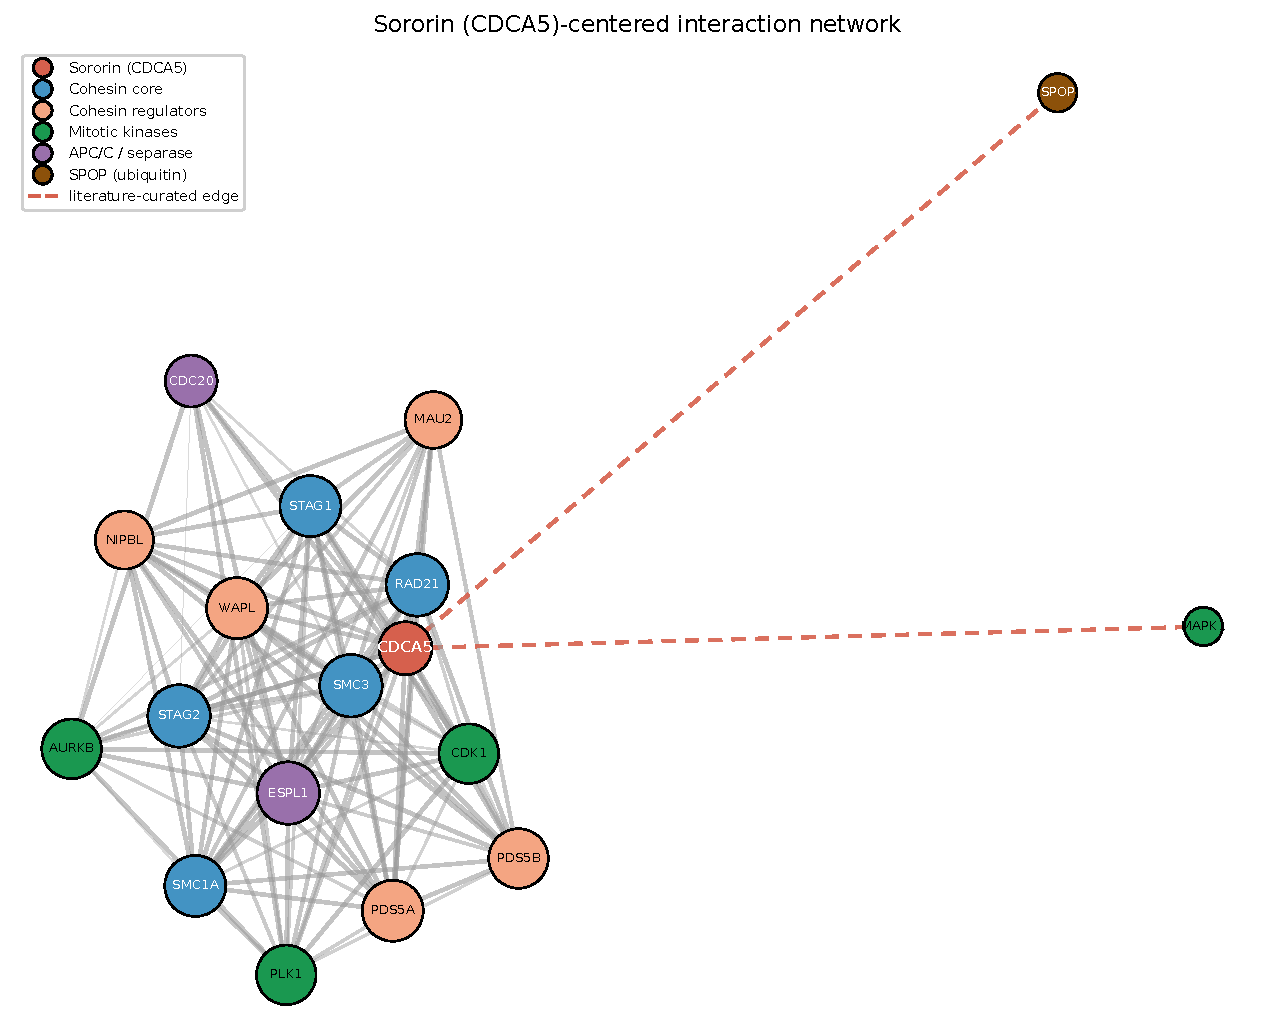
\includegraphics[width=0.86\textwidth]{Fig1_interaction_network.pdf}
\caption{\textbf{Sororin (CDCA5)-centred interaction network.} Nodes are proteins coloured by functional class and edges are STRING associations (combined score $\ge 0.4$); edge width and opacity scale with confidence. Node size scales with degree. Dashed red edges denote literature-curated regulatory interactions (ERK2/MAPK1 and SPOP) that are absent from the high-confidence STRING neighbourhood. The STRING module is a dense cohesin-centred graph (16 nodes, 107 edges, density $=0.89$) with Sororin as a high-degree hub; ERK2/MAPK1 and SPOP are shown as two additional literature-curated nodes.}
\label{fig:net}
\end{figure}

\begin{table}[htbp]
\centering
\caption{\textit{High-confidence STRING partners of Sororin (CDCA5) and their functional class. Combined scores are STRING confidence values in $[0,1]$; the full module comprises 16 nodes and 107 edges (density $=0.89$).}}
\label{tab:net}
\small
\begin{tabular}{llc}
\toprule
Partner & Functional class & STRING combined score \\
\midrule
PDS5A & Cohesin regulator (PDS5) & 0.999 \\
WAPL  & Cohesin regulator (release) & 0.998 \\
SMC3  & Cohesin core & 0.994 \\
PDS5B & Cohesin regulator (PDS5) & 0.990 \\
RAD21 & Cohesin core (kleisin) & 0.988 \\
CDK1  & Mitotic kinase & 0.979 \\
STAG2 & Cohesin core & 0.977 \\
STAG1 & Cohesin core & 0.975 \\
SMC1A & Cohesin core & 0.973 \\
NIPBL & Cohesin loader & 0.970 \\
AURKB & Mitotic kinase & 0.968 \\
CDC20 & APC/C activator & 0.938 \\
ESPL1 & Separase & 0.930 \\
MAU2  & Cohesin loader & 0.917 \\
PLK1  & Mitotic kinase & 0.893 \\
\midrule
ERK2 (MAPK1) & Cross-talk (literature) & --- \\
SPOP & Ubiquitin ligase (literature) & --- \\
\bottomrule
\end{tabular}
\end{table}

\begin{figure}[htbp]
\centering
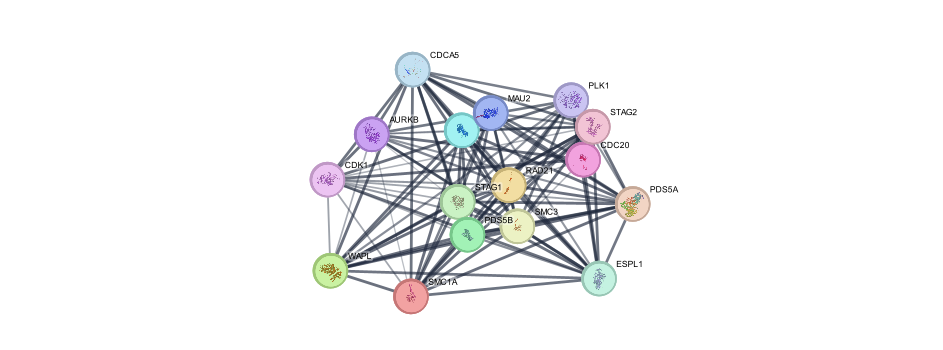
\includegraphics[width=0.82\textwidth]{Fig5_cytoscape_network.png}
\caption{\textbf{Independent reconstruction of the cohesin module in Cytoscape.} The same 16-protein module was retrieved from STRING and rendered with the Cytoscape stringApp; node glyphs show STRING structure previews and edge thickness scales with the combined score. Cytoscape's network analyzer returned the same topology as the custom pipeline (16 nodes, 107 edges, density $0.892$, clustering coefficient $0.925$), with CDCA5 a maximally connected node (degree $15$).}
\label{fig:cyto}
\end{figure}

\begin{table}[htbp]
\centering
\caption{\textit{Representative functional enrichment of the 16-protein module (stringApp, whole-genome background, FDR $<0.05$). The module shows a STRING PPI enrichment $p<10^{-16}$; the terms below are the most significant in each source, all reflecting sister-chromatid cohesion and cell-cycle function.}}
\label{tab:enrich}
\small
\begin{tabular}{lllc}
\toprule
Source & Term & Description & FDR \\
\midrule
GO Process & GO:0007062 & Sister chromatid cohesion & $1.4\times10^{-24}$ \\
GO Process & GO:0000819 & Sister chromatid segregation & $2.3\times10^{-24}$ \\
GO Process & GO:0000278 & Mitotic cell cycle & $1.2\times10^{-18}$ \\
GO Component & GO:0098687 & Chromosomal region & $7.0\times10^{-15}$ \\
KEGG & hsa04110 & Cell cycle & $6.1\times10^{-14}$ \\
Reactome & HSA-2500257 & Resolution of sister chromatid cohesion & $1.7\times10^{-23}$ \\
Reactome & HSA-2468052 & Establishment of sister chromatid cohesion & $4.4\times10^{-22}$ \\
\bottomrule
\end{tabular}
\end{table}

\FloatBarrier
\subsection{Interaction determinants map to disordered regions: Sororin as a fuzzy hub}
Having established the partners, we next asked in what structural context they are bound, i.e.\ whether the sequence elements that mediate these interactions are folded or intrinsically disordered. Running IUPred2 and ANCHOR2 over the full 252-residue sequence showed that Sororin is predominantly disordered: $61.5\%$ of residues had IUPred2 $>0.5$ (mean score $0.61$), organised into three long disordered regions (residues 1--48, 72--142 and 199--222) separated by short segments of transient structure (Figure~\ref{fig:dis}). The only region with a robustly folded signature was the C-terminal conserved Sororin domain (residues 230--252; mean IUPred2 $0.31$, $0\%$ disordered), which is precisely the element shown experimentally to be required for cohesion and cohesin association \citep{wu2011}.

Superimposing the experimentally defined interaction determinants onto this profile revealed that they lie, almost without exception, in disordered segments (Table~\ref{tab:map}). The APC/C-recognition KEN box (residues 88--90) sits in a fully disordered region (mean IUPred2 $0.64$); the ERK2 phospho-acceptor Ser209 lies on a disorder peak within the 199--222 IDR (IUPred2 $0.74$); and the PDS5-binding FGF motif (residues 166--168) maps to a short, locally ordered dip inside otherwise disordered sequence---the signature of a short linear motif, which becomes ordered only when it binds \citep{fuxreiter2007,davey2012}. Consistent with a binding-competent disordered protein, ANCHOR2 predicted several disordered-binding segments spanning the N-terminal, central and C-terminal IDRs (residues 1--70, 78--118, 127--153, 198--204 and 227--240), which collectively cover the KEN box, the phospho-cluster and the region approaching the FGF motif. The contrast between the folded C-terminal domain and the disordered location of the KEN box, the FGF motif and the phospho-sites indicates that Sororin engages its partners chiefly through disordered segments and short linear motifs rather than through a globular interface---that is, as a fuzzy interaction hub, whose recognition elements can be tuned by modification.

We tested this fuzzy-hub interpretation directly with FuzPred, a sequence-based predictor of context-dependent binding behaviour built specifically to quantify fuzziness \citep{miskei2020,horvath2020}. Consistent with a fuzzy hub, Sororin was predicted to engage partners predominantly without folding: the median disorder-to-order probability was only $0.40$, $62\%$ of residues favoured disorder-to-disorder (fuzzy) binding, and $68\%$ showed a high multiplicity of binding modes (MBM $>0.65$), i.e.\ the capacity to bind in several alternative modes (Figure~\ref{fig:fuz}). FuzPred classified $63\%$ of the sequence as context-dependent and only $25\%$ as fold-on-binding, the latter confined to three short segments including the C-terminal Sororin domain (residues 231--248). Mapping the interaction determinants onto this landscape reproduced the division of labour identified above: the C-terminal domain is fold-on-binding (pDO $0.66$), whereas the PDS5-binding FGF motif (pDO $0.34$, pDD $0.66$, MBM $0.70$) and the ERK2 site Ser209 (pDO $0.33$, MBM $0.80$) lie in fuzzy, multi-mode regions, while the APC/C KEN box is the expected exception, predicted to fold upon binding (pDO $0.87$) as befits a degron recognised by a folded receptor. FuzPred additionally annotated the two Pfam families of Sororin---the middle region (89--214) and the C-terminal region (229--252)---of which only the C-terminal family coincides with the ordered, fold-on-binding segment. A method built specifically to detect fuzziness therefore returns the same picture, supporting the fuzzy-hub description independently.

\begin{figure}[htbp]
\centering
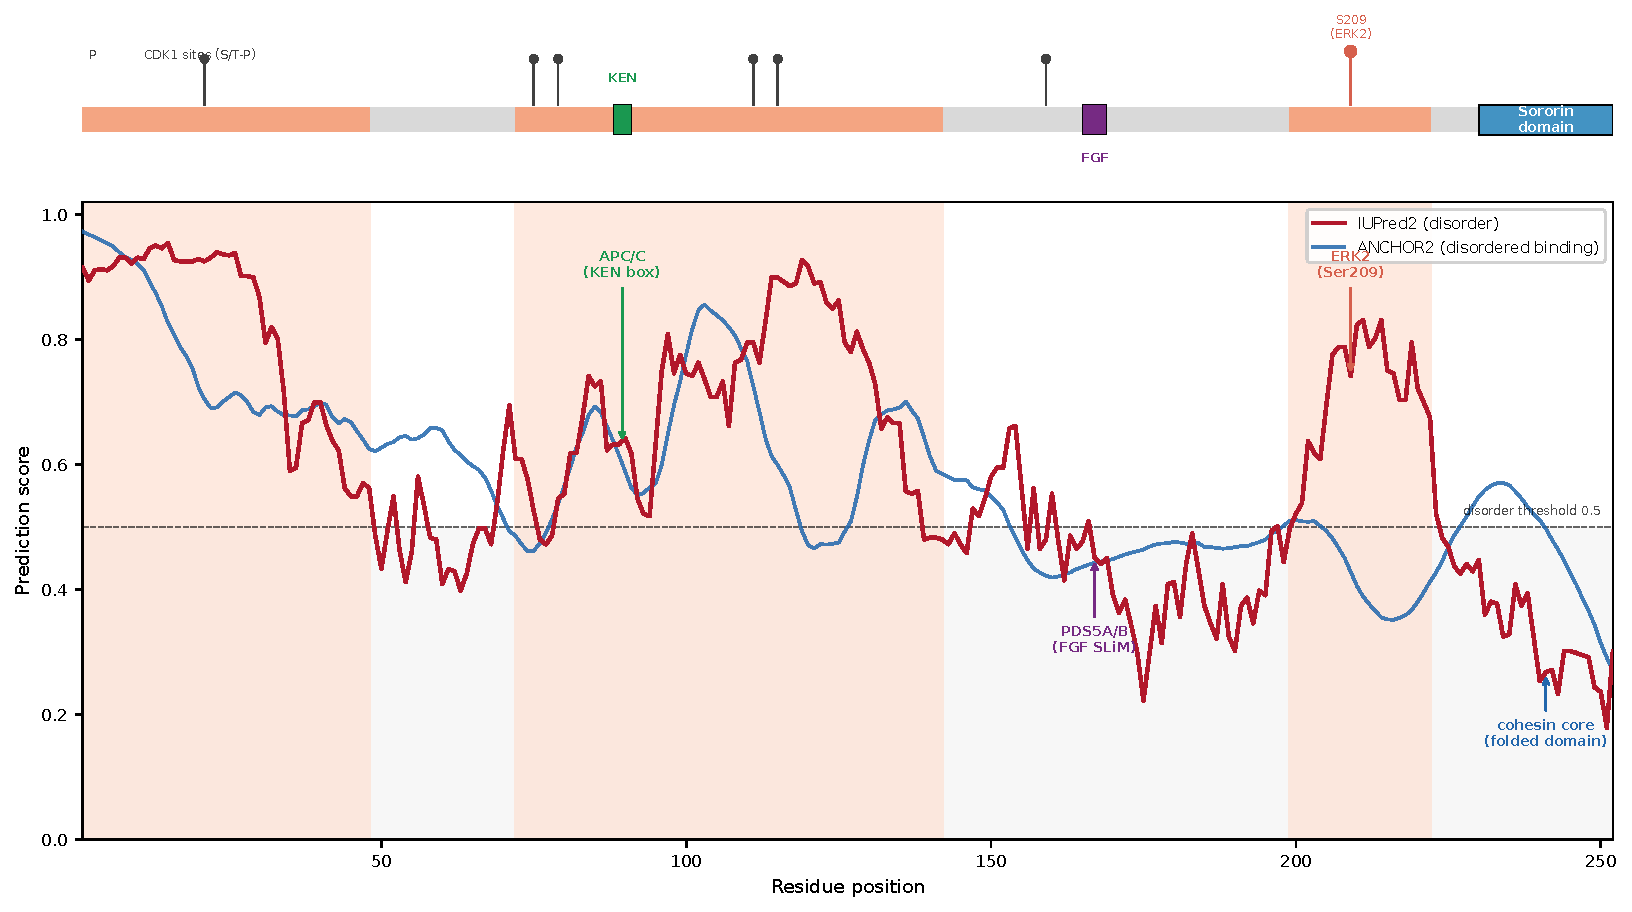
\includegraphics[width=\textwidth]{Fig2_disorder_map.pdf}
\caption{\textbf{Disorder landscape of Sororin with interaction determinants annotated.} \textit{Top,} domain architecture: three intrinsically disordered regions (orange; UniProt 1--48, 72--142, 199--222), the folded C-terminal Sororin domain (blue), the KEN box and FGF motif, and proline-directed (S/T-P) phospho-sites (lollipops; the ERK2 target Ser209 in red). Bottom, per-residue IUPred2 disorder (red) and ANCHOR2 disordered-binding (blue) scores; the dashed line is the disorder threshold ($0.5$) and shaded bands mark the annotated IDRs. The APC/C KEN box and the ERK2 site Ser209 fall in disordered regions, the PDS5-binding FGF motif is a short ordered dip embedded in disorder, and the only folded element is the C-terminal Sororin domain.}
\label{fig:dis}
\end{figure}

\begin{figure}[htbp]
\centering
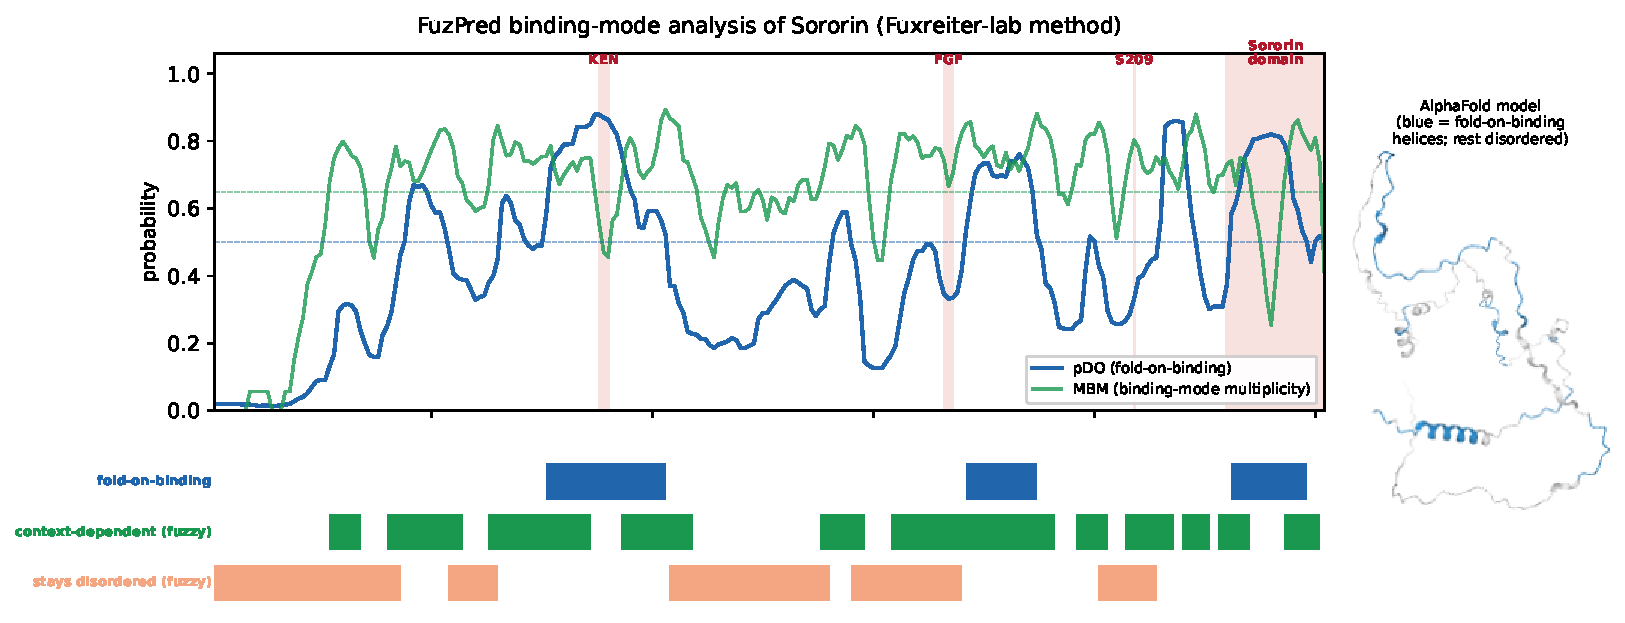
\includegraphics[width=\textwidth]{Fig6_fuzpred.pdf}
\caption{\textbf{FuzPred binding-mode analysis of Sororin.} Left (top), per-residue probability of disorder-to-order (fold-on-binding) binding (pDO, blue) and multiplicity of binding modes (MBM, green); dashed lines mark the $0.5$ and $0.65$ references and red bands the interaction determinants. Left (bottom), FuzPred region classification in three overlapping tracks (fold-on-binding, context-dependent, and stays-disordered). Right, the AlphaFold model (fold-on-binding helices in blue, the remainder disordered). Most of the protein is context-dependent and multi-mode; only three short segments, including the C-terminal domain, fold on binding.}
\label{fig:fuz}
\end{figure}

\begin{table}[htbp]
\centering
\caption{\textit{Mapping of Sororin interaction determinants onto the predicted disorder landscape. Region disorder is the mean IUPred2 score and the fraction of residues with IUPred2 $>0.5$ over the indicated residues.}}
\label{tab:map}
\small
\begin{tabular}{lllcl}
\toprule
Determinant & Residues & Partner / role & Mean IUPred2 (\% dis.) & Structural context \\
\midrule
N-terminal IDR & 1--48 & loading / regulation & 0.82 (100\%) & disordered \\
KEN box & 88--90 & APC/C (degradation) & 0.64 (100\%) & disordered \\
Central IDR & 72--142 & phospho-cluster & 0.70 (90\%) & disordered \\
FGF motif & 166--168 & PDS5A/B (cohesion) & 0.47 (33\%) & SLiM / ordered dip in IDR \\
Ser209 site & 199--222 & ERK2 (phosphorylation) & 0.71 (96\%) & disordered \\
Sororin domain & 230--252 & cohesin core association & 0.31 (0\%) & folded \\
\bottomrule
\end{tabular}
\end{table}

\FloatBarrier
\subsection{The phospho-interactome and SPOP ubiquitin cross-talk act through the disordered chain}
Finally, we asked how the disordered interactome of Sororin is switched, by locating its regulatory modifications on the same profile. Of the thirteen curated phospho-sites, seven are proline-directed (S/T-P) and therefore candidate substrates of the proline-directed kinases CDK1 and ERK: Ser21, Ser75, Ser79, Thr111, Thr115, Thr159 and Ser209 (Table~\ref{tab:phos}). None lies in the folded C-terminal domain: six fall within the three intrinsically disordered regions and the seventh, Thr159, in the short linker immediately preceding the FGF motif. They flank the very determinants identified above: the central cluster (Ser75--Thr115) surrounds the KEN box, Thr159 abuts the PDS5-binding FGF motif, and Ser209 sits in the C-terminal IDR. This co-localisation offers a sequence-level rationale for the established regulatory logic, in which mitotic phosphorylation of Sororin by CDK1 (assisted by Aurora B) displaces it from PDS5 and relieves WAPL inhibition, dissolving arm cohesion \citep{nishiyama2013,dreier2011}: because the PDS5-binding FGF motif is a short element embedded in a disordered, heavily phosphorylatable context, phosphorylation of the surrounding chain can switch the interaction off without disrupting a folded domain, as expected for a fuzzy complex \citep{tompa2008,fuxreiter2018}.

The same disordered architecture accommodates the two cancer-associated inputs. The ERK2/MAPK site Ser209, reported to be phosphorylated during lung carcinogenesis \citep{nguyen2010}, lies at one of the most disordered positions in the protein, and so in a readily accessible context for a proline-directed kinase; and the SPOP-dependent degradation that controls CDCA5 levels in prostate cancer \citep{zhang2021} requires a SPOP-binding degron, a class of short motif that is typically presented from disordered, accessible sequence. Mitotic inactivation, oncogenic ERK phosphorylation and SPOP-mediated turnover are thus all concentrated on the same disordered regions, consistent with a fuzzy hub whose interactions are toggled by post-translational modification.

\begin{table}[htbp]
\centering
\caption{\textit{Proline-directed (S/T-P) phosphorylation sites of Sororin and their context. Six of the seven candidate CDK1/ERK sites lie within intrinsically disordered regions and the seventh (Thr159) in the short linker preceding the FGF motif; none is in the folded C-terminal domain.}}
\label{tab:phos}
\small
\begin{tabular}{llll}
\toprule
Site & Motif (S/T-P) & Disordered region & Reported role / kinase \\
\midrule
Ser21  & SP & 1--48 (N-terminal IDR)   & CDK1 consensus \citep{dreier2011} \\
Ser75  & SP & 72--142 (central IDR)    & CDK1 consensus \citep{dreier2011} \\
Ser79  & SP & 72--142 (central IDR)    & ERK/MAPK site \citep{nguyen2010} \\
Thr111 & TP & 72--142 (central IDR)    & CDK1 consensus \citep{dreier2011} \\
Thr115 & TP & 72--142 (central IDR)    & CDK1 consensus \citep{dreier2011} \\
Thr159 & TP & linker (pre-FGF)         & CDK1 consensus \citep{dreier2011} \\
Ser209 & SP & 199--222 (C-terminal IDR)& ERK2 site, lung cancer \citep{nguyen2010} \\
\bottomrule
\end{tabular}
\end{table}

\FloatBarrier
\subsection{Predicted short linear motifs anchor specific network edges to the disordered chain}
The disorder profile shows that Sororin's interaction determinants sit in disordered sequence, but disorder alone does not specify which partner binds where. To close this gap we screened the full sequence against the ELM resource and retained the predictions whose motif class corresponds to a partner already present in the network (Table~\ref{tab:elm}, Figure~\ref{fig:elm}). ELM independently recovered the annotated KEN box (residues 87--91, flagged by ELM as an experimentally validated instance) as an APC/C-recognition (DEG\_APCC\_KENBOX\_2) motif, matching the UniProt annotation (88--90) to within one residue. It further identified two SPOP-binding-consensus degrons (DEG\_SPOP\_SBC\_1) at residues 122--126 and 155--159, providing a concrete sequence-level candidate for the SPOP-dependent degradation reported in prostate cancer \citep{zhang2021}, which the network alone could only represent as an edge. A generic MAPK docking motif (DOC\_MAPK\_gen\_1, residues 77--84) was found immediately adjacent to the reported ERK/MAPK phospho-site Ser79 \citep{nguyen2010}, giving ERK2 a plausible physical docking element in addition to its phospho-acceptor site, and a PLK1 phosphorylation motif (MOD\_Plk\_1) was identified at residues 201--207, close to the ERK2 site Ser209, consistent with PLK1's role as one of the mitotic kinases in the high-confidence STRING module. Finally, nine occurrences of the generic proline-directed kinase motif (MOD\_ProDKin\_1) recapitulated the same cluster of CDK1 candidate sites as the manual S/T-P classification of Section~3.3, here obtained through ELM's curated motif pattern rather than a hand-coded rule, providing a consistency check between the two approaches.

Of these fourteen network-linked motifs, eleven (79\%) are majority disordered (mean IUPred2 $0.65$, mean $67\%$ disordered over the motif window for the CDK1 cluster); the exceptions are the second SPOP degron and one CDK1 site, which fall in the short, partially ordered linker adjoining the FGF motif, in the same region as the outlier phospho-site Thr159 identified in Section~3.3. Rather than reporting disorder as a general property, this analysis proposes a specific candidate motif for four of the five partners examined (APC/C, SPOP, ERK2/MAPK1 and PLK1), each lying predominantly, though not exclusively, within a disordered region.

\begin{figure}[htbp]
\centering
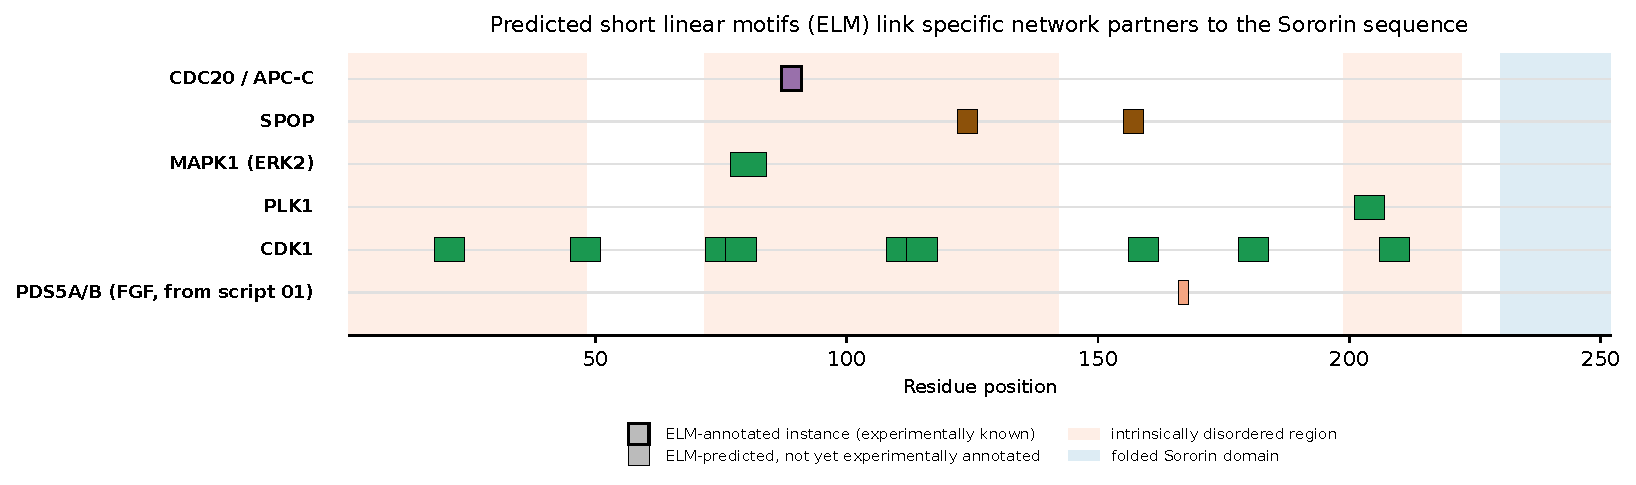
\includegraphics[width=\textwidth]{Fig3_motif_network_map.pdf}
\caption{\textbf{Predicted short linear motifs link specific network partners to the Sororin sequence.} Each row is a network partner (or literature-curated node); coloured blocks mark the residue range of an ELM-predicted motif for that partner. Blocks are coloured by the partner's functional class, matching the node colours in Figure~\ref{fig:net}: green for mitotic kinases (CDK1, ERK2/MAPK1 and PLK1, which therefore share one colour), purple for APC/C, brown for SPOP (ubiquitin), and salmon for cohesin regulators (PDS5A/B). Thick-edged blocks are ELM-annotated (experimentally documented) instances; thin-edged blocks are ELM predictions without a prior experimental annotation. Shaded bands as in Figure~\ref{fig:dis}: orange for the intrinsically disordered regions, blue for the folded C-terminal domain. The FGF motif (UniProt annotation, not an ELM class) is shown for reference.}
\label{fig:elm}
\end{figure}

\begin{table}[htbp]
\centering
\caption{\textit{Curated, network-linked short linear motifs predicted by ELM. The CDK1 row summarises the nine MOD\_ProDKin\_1 hits (individual ranges: 18--24, 45--51, 72--78, 76--82, 108--114, 112--118, 156--162, 178--184, 206--212); all other rows are single motifs. Disorder statistics are the mean IUPred2 score and \% of residues with IUPred2 $>0.5$ over the motif window(s), from the same profile as Table~\ref{tab:map}.}}
\label{tab:elm}
\small
\begin{tabular}{lllccl}
\toprule
ELM class & Residues & Partner & Mean IUPred2 & \% dis. & Annotated? \\
\midrule
DEG\_APCC\_KENBOX\_2 & 87--91 & CDC20 / APC-C & 0.63 & 100\% & yes (ELM) \\
DEG\_SPOP\_SBC\_1 & 122--126 & SPOP & 0.85 & 100\% & no \\
DEG\_SPOP\_SBC\_1 & 155--159 & SPOP & 0.51 & 40\% & no \\
DOC\_MAPK\_gen\_1 & 77--84 & MAPK1 (ERK2) & 0.59 & 75\% & no \\
MOD\_Plk\_1 & 201--207 & PLK1 & 0.67 & 100\% & no \\
MOD\_ProDKin\_1 (9 sites) & see caption & CDK1 & 0.65 & 67\% & no \\
\bottomrule
\end{tabular}
\end{table}

\FloatBarrier
\subsection{Secondary-structure prediction and a second disorder predictor recover the single folded element}
Finally, we asked whether the folded/disordered partition inferred from IUPred2 is matched by an actual secondary-structure assignment and by an independent disorder predictor. PSIPRED~4.0 assigned only $18.7\%$ of the sequence to helix and $3.2\%$ to strand, leaving $78.2\%$ as coil (Figure~\ref{fig:ss}), and placed its only two extended helices at residues 133--145 and, most prominently, 225--245; the latter lies within the conserved C-terminal Sororin domain (residues 230--252), which was $70\%$ helix and $83\%$ ordered secondary structure overall (Table~\ref{tab:ss}). DISOPRED3 independently classified $63.9\%$ of the protein as disordered, closely matching the IUPred2 value of $61.5\%$ obtained by a different method (Section~3.2), and assigned the C-terminal Sororin domain $0\%$ disorder. The two predictors therefore converge on the same architecture: the C-terminal domain is the single element that is simultaneously ordered in secondary structure ($83\%$ H/E) and non-disordered ($0\%$), whereas the three intrinsically disordered regions are almost entirely coil ($79$--$100\%$) and predominantly disordered ($46$--$100\%$ by DISOPRED3). The interaction motifs mapped, as before, outside the folded domain: the KEN box, the MAPK docking motif and both SPOP degrons fell in coil, and the PDS5-binding FGF motif was assigned coil with a locally low DISOPRED3 disorder score, matching the ordered SLiM dip identified in Section~3.2 \citep{fuxreiter2007}. Both methods therefore recover the one experimentally supported folded element \citep{wu2011} and assign no comparable ordered structure elsewhere.

Because secondary-structure predictors differ in how much information they use, we repeated the assignment with GOR~IV \citep{garnier1996}, a single-sequence information-theory method, and compared it with the profile-based PSIPRED (Table~\ref{tab:ss}). The two agree where the claim of this work rests: GOR~IV assigns the C-terminal Sororin domain (residues 230--252) $83\%$ helix and only $4\%$ coil---an even stronger helical signal than PSIPRED ($70\%$ helix)---and its longest predicted helix, residues 223--248, coincides with that domain, so the single folded element is recovered by both. Both methods likewise call the KEN box and the PLK1 motif entirely coil, and neither assigns helix to the N-terminal IDR (GOR~IV $0\%$ helix, $94\%$ coil). The methods diverge, as expected, in the disordered regions: over the whole protein GOR~IV predicts $34.9\%$ helix, $6.7\%$ strand and $58.3\%$ coil, against $18.7\%$, $3.2\%$ and $78.2\%$ for PSIPRED, the excess helix falling almost entirely inside the intrinsically disordered regions (central IDR $39\%$ helix by GOR~IV versus $21\%$ by PSIPRED). This is the documented behaviour of single-sequence propensity methods, which over-predict regular secondary structure in low-complexity and disordered sequence because they cannot exploit the evolutionary conservation signal that a profile-based predictor obtains from a multiple-sequence alignment \citep{jones1999}. The comparison therefore does not weaken the disorder-centred picture: the two predictors converge on the folded C-terminal domain and on the coil assignment of the interaction motifs, and their only substantial disagreement is a helix excess in precisely the regions that IUPred2, DISOPRED3 and FuzPred independently classify as disordered---consistent with helical propensity in a disordered chain that is realised only transiently, rather than a stable fold.

\begin{figure}[htbp]
\centering
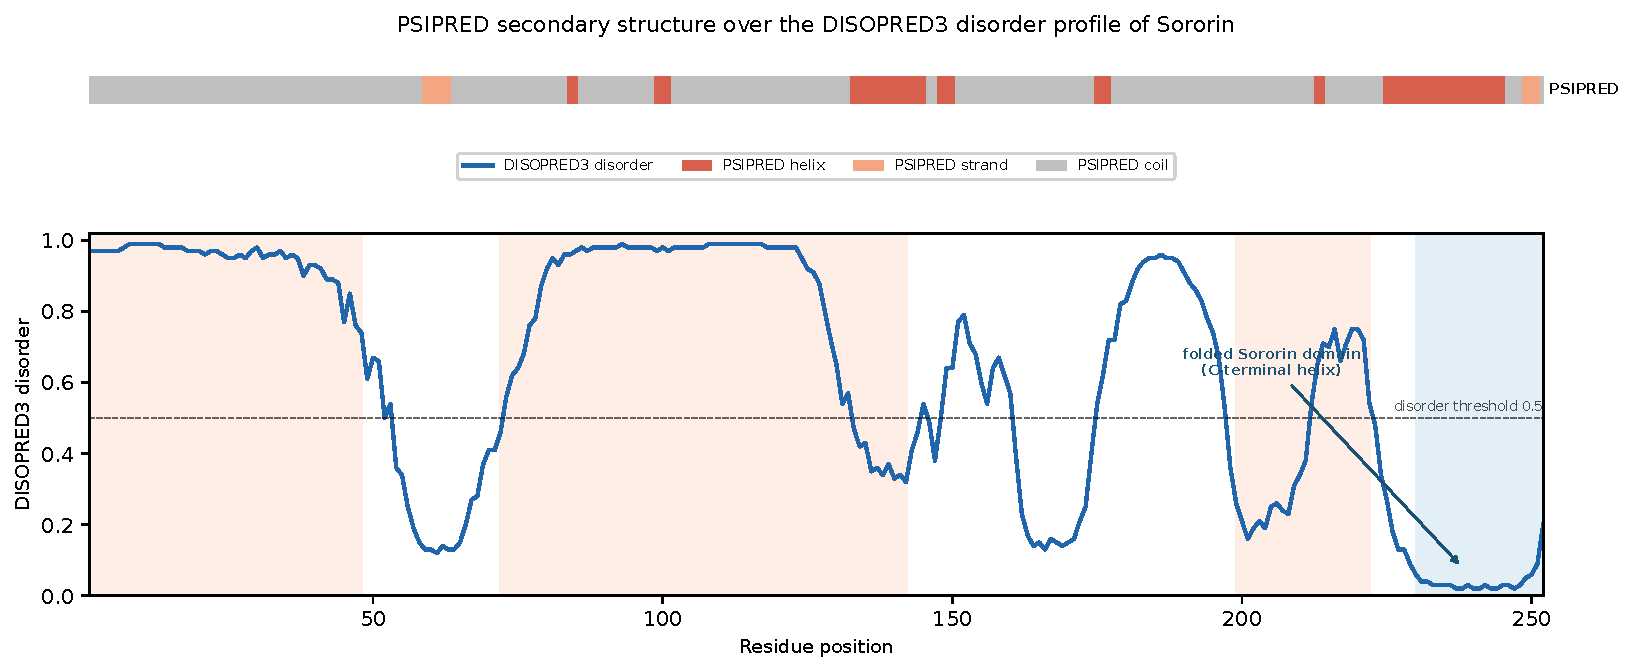
\includegraphics[width=\textwidth]{Fig4_secondary_structure.pdf}
\caption{\textbf{PSIPRED secondary structure over the DISOPRED3 disorder profile of Sororin.} Top, per-residue PSIPRED assignment (red, helix; orange, strand; grey, coil). Bottom, DISOPRED3 per-residue disorder with the $0.5$ threshold (dashed); shaded bands as in Figure~\ref{fig:dis}: orange, the three intrinsically disordered regions; blue, the folded C-terminal Sororin domain. The only extended ordered element is the C-terminal helix (residues 225--245), which coincides with the deep DISOPRED3 disorder minimum; the remainder of the chain is coil and predicted disordered.}
\label{fig:ss}
\end{figure}

\begin{table}[htbp]
\centering
\caption{\textit{Secondary structure and disorder over the annotated regions and network-linked motifs. Values are the percentage of residues in each region assigned to helix, strand or coil by the profile-based PSIPRED and by the single-sequence GOR~IV, and to the disordered state by DISOPRED3. Only the C-terminal Sororin domain is ordered by every measure; GOR~IV's excess helix is confined to the intrinsically disordered regions.}}
\label{tab:ss}
\small
\begin{tabular}{llcccccc}
\toprule
 & & \multicolumn{3}{c}{PSIPRED (profile)} & \multicolumn{2}{c}{GOR~IV (single-seq.)} & DISOPRED3 \\
\cmidrule(lr){3-5}\cmidrule(lr){6-7}\cmidrule(lr){8-8}
Region & Residues & \% helix & \% strand & \% coil & \% helix & \% coil & \% disordered \\
\midrule
N-terminal IDR & 1--48 & 0 & 0 & 100 & 0 & 94 & 100 \\
Central IDR & 72--142 & 21 & 0 & 79 & 39 & 58 & 85 \\
C-terminal IDR & 199--222 & 8 & 0 & 92 & 38 & 62 & 46 \\
KEN box (APC/C) & 88--90 & 0 & 0 & 100 & 0 & 100 & 100 \\
MAPK docking (ERK2) & 77--84 & 12 & 0 & 88 & 38 & 62 & 100 \\
SPOP degron 1 & 122--126 & 0 & 0 & 100 & 40 & 60 & 100 \\
FGF motif (PDS5A/B) & 166--168 & 0 & 0 & 100 & 0 & 67 & 0 \\
PLK1 motif & 201--207 & 0 & 0 & 100 & 0 & 100 & 0 \\
Sororin domain & 230--252 & 70 & 13 & 17 & 83 & 4 & 0 \\
\midrule
\textit{whole protein} & 1--252 & \textit{18.7} & \textit{3.2} & \textit{78.2} & \textit{34.9} & \textit{58.3} & \textit{63.9} \\
\bottomrule
\end{tabular}
\end{table}

\FloatBarrier
\section{Discussion and Conclusion}

We set out to determine whether Sororin engages its partners through folded domains or through intrinsically disordered regions, and whether the modifications that toggle those interactions are located in disordered sequence. Integrating a cohesin-centred interaction network with per-residue disorder and binding predictions and with the experimentally defined interaction motifs, we found that Sororin is a small, high-confidence hub of a dense cohesin module (density $0.89$) that is itself $\sim\!62\%$ intrinsically disordered; that its APC/C, PDS5 and ERK2 determinants all reside in disordered segments while only the short C-terminal domain is folded; and that its seven proline-directed phospho-sites lie outside the folded C-terminal domain, in the disordered regions and adjoining linker surrounding those determinants; and, going beyond disorder as a general property, that an independent linear-motif prediction anchors four of the five scrutinised network partners (APC/C, SPOP, ERK2/MAPK1, PLK1) to a specific short sequence element, predominantly but not exclusively within the disordered regions. Together these observations indicate that the Sororin interactome is built on disorder, and that where a partner-specific claim can be made, it is a short linear motif embedded in that disorder---rather than disorder in the abstract---that explains the edge.

This picture fits the established biology of Sororin. Mitotic phosphorylation by Cdk1 and Aurora B is known to remove Sororin from PDS5 and activate WAPL \citep{nishiyama2013,dreier2011}; that the proline-directed sites cluster in the disordered regions flanking the PDS5-binding motif suggests the switch is implemented on a disordered, modification-dense chain rather than a rigid interface. The crystal structure of PDS5B bound to the shared FGF peptide of WAPL and Sororin \citep{ouyang2016} shows that contact being made by a short motif presented from otherwise unstructured sequence, matching the locally ordered dip we observe there. Finally, the requirement of the conserved C-terminal element for cohesion \citep{wu2011} matches the single folded region in our profile, suggesting a division of labour between a disordered regulatory body and a compact functional C-terminus.

The framework also accommodates the two cancer-associated regulators that were peripheral in the network. The ERK2 site Ser209, phosphorylated in lung carcinogenesis \citep{nguyen2010}, is among the most disordered residues of the protein and lies close to a predicted PLK1 motif and, further upstream, to a predicted MAPK docking motif adjoining the second ERK site Ser79. The SPOP-dependent degradation that controls CDCA5 abundance in prostate cancer \citep{zhang2021} depends on a degron, which is typically presented from accessible, disordered sequence---consistent with the two SPOP motifs predicted here at residues 122--126 and 155--159.

Placing these inputs on the disorder map suggests a unifying model. Sororin is a fuzzy interaction hub \citep{tompa2008,fuxreiter2018}, in line with the known enrichment of disorder among interaction hubs \citep{haynes2006} and independently supported by FuzPred \citep{miskei2020,horvath2020}. A mostly disordered chain displays a set of short linear motifs---the KEN degron, the FGF motif, two candidate SPOP degrons and a MAPK docking motif---interleaved with proline-directed phospho-sites, so that kinases and ubiquitin ligases can switch individual contacts without remodelling a folded core. We propose that this disorder is what makes Sororin an efficient, multiply-regulated node, and that it works through a small, enumerable set of linear motifs rather than through disorder alone.

Three limitations temper these conclusions. First, disorder and binding propensities are predictions; although IUPred2 and ANCHOR2 are well validated and the folded C-terminal domain and the FGF dip are recovered as expected, direct structural confirmation of the bound states would strengthen the fuzzy-hub interpretation. Second, the ERK2 and SPOP edges rest on individual studies and are not yet part of curated interaction databases, so their network context is provisional. Third, the ELM motif predictions reported here are, with the exception of the KEN box, sequence-based predictions without direct experimental validation in Sororin itself; the SPOP degrons and MAPK docking motif in particular should be considered testable hypotheses---for example by mutagenesis of the SPOP-binding-consensus residues and assessment of CDCA5 turnover---rather than established interaction sites.

In conclusion, a disorder-centred systems analysis indicates that Sororin functions as a fuzzy cohesin hub whose partners---the cohesin core, PDS5A/B and WAPL, the APC/C, and the cancer-linked ERK2 and SPOP pathways---are engaged and switched through intrinsically disordered regions and short linear motifs rather than a globular scaffold; independent ELM motif prediction anchors four of these five partners to a specific, enumerable sequence element rather than to disorder as a general property, providing candidate SPOP degron and MAPK docking sites that the network alone could not localise. Looking forward, the model makes testable predictions: phospho-mimetic substitutions within the disordered central and C-terminal regions should quantitatively tune PDS5 binding and Sororin turnover, and mutation of the predicted SPOP-binding-consensus residues (122--126 or 155--159) should measurably alter CDCA5 turnover if either is the operative degron. Experimental dissection of these disordered elements and their motifs, ideally combined with an ensemble structural description of the Sororin--PDS5 complex, would test whether targeting a disordered hub offers a route to modulating cohesion in cancers where CDCA5 is over-expressed.

\begin{thebibliography}{99}
\setlength{\itemsep}{1pt}

\bibitem[Nasmyth and Haering(2009)]{nasmyth2009} Nasmyth K, Haering CH. Cohesin: its roles and mechanisms. \textit{Annu Rev Genet}. 2009;43:525--558. doi:10.1146/annurev-genet-102108-134233.

\bibitem[Rankin et al.(2005)]{rankin2005} Rankin S, Ayad NG, Kirschner MW. Sororin, a substrate of the anaphase-promoting complex, is required for sister chromatid cohesion in vertebrates. \textit{Mol Cell}. 2005;18(2):185--200. doi:10.1016/j.molcel.2005.03.017.

\bibitem[Nishiyama et al.(2010)]{nishiyama2010} Nishiyama T, Ladurner R, Schmitz J, et al. Sororin mediates sister chromatid cohesion by antagonizing Wapl. \textit{Cell}. 2010;143(5):737--749. doi:10.1016/j.cell.2010.10.031.

\bibitem[Dreier et al.(2011)]{dreier2011} Dreier MR, Bekier ME 2nd, Taylor WR. Regulation of sororin by Cdk1-mediated phosphorylation. \textit{J Cell Sci}. 2011;124(Pt 17):2976--2987. doi:10.1242/jcs.085431.

\bibitem[Wu et al.(2011)]{wu2011} Wu FM, Nguyen JV, Rankin S. A conserved motif at the C terminus of sororin is required for sister chromatid cohesion. \textit{J Biol Chem}. 2011;286(5):3579--3586. doi:10.1074/jbc.M110.196758.

\bibitem[Nishiyama et al.(2013)]{nishiyama2013} Nishiyama T, Sykora MM, Huis in 't Veld PJ, Mechtler K, Peters JM. Aurora B and Cdk1 mediate Wapl activation and release of acetylated cohesin from chromosomes by phosphorylating Sororin. \textit{Proc Natl Acad Sci USA}. 2013;110(33):13404--13409. doi:10.1073/pnas.1305020110.

\bibitem[Ouyang et al.(2016)]{ouyang2016} Ouyang Z, Zheng G, Tomchick DR, Luo X, Yu H. Structural basis and IP6 requirement for Pds5-dependent cohesin dynamics. \textit{Mol Cell}. 2016;62(2):248--259. doi:10.1016/j.molcel.2016.02.033.

\bibitem[Nguyen et al.(2010)]{nguyen2010} Nguyen MH, Koinuma J, Ueda K, et al. Phosphorylation and activation of cell division cycle associated 5 by mitogen-activated protein kinase play a crucial role in human lung carcinogenesis. \textit{Cancer Res}. 2010;70(13):5337--5347. doi:10.1158/0008-5472.CAN-09-4372.

\bibitem[Luo et al.(2021)]{zhang2021} Luo Z, Wang J, Zhu Y, et al. SPOP promotes CDCA5 degradation to regulate prostate cancer progression via the AKT pathway. \textit{Neoplasia}. 2021;23(10):1037--1047. doi:10.1016/j.neo.2021.08.002.

\bibitem[Tompa and Fuxreiter(2008)]{tompa2008} Tompa P, Fuxreiter M. Fuzzy complexes: polymorphism and structural disorder in protein-protein interactions. \textit{Trends Biochem Sci}. 2008;33(1):2--8. doi:10.1016/j.tibs.2007.10.003.

\bibitem[Miskei et al.(2020)]{miskei2020} Miskei M, Horvath A, Vendruscolo M, Fuxreiter M. Sequence-based prediction of fuzzy protein interactions. \textit{J Mol Biol}. 2020;432(7):2289--2303. doi:10.1016/j.jmb.2020.02.017.

\bibitem[Horvath et al.(2020)]{horvath2020} Horvath A, Miskei M, Ambrus V, Vendruscolo M, Fuxreiter M. Sequence-based prediction of protein binding mode landscapes. \textit{PLoS Comput Biol}. 2020;16(5):e1007864. doi:10.1371/journal.pcbi.1007864.

\bibitem[Fuxreiter et al.(2007)]{fuxreiter2007} Fuxreiter M, Tompa P, Simon I. Local structural disorder imparts plasticity on linear motifs. \textit{Bioinformatics}. 2007;23(8):950--956. doi:10.1093/bioinformatics/btm035.

\bibitem[Fuxreiter(2018)]{fuxreiter2018} Fuxreiter M. Fuzziness in protein interactions---a historical perspective. \textit{J Mol Biol}. 2018;430(16):2278--2287. doi:10.1016/j.jmb.2018.02.015.

\bibitem[Wright and Dyson(2015)]{wright2015} Wright PE, Dyson HJ. Intrinsically disordered proteins in cellular signalling and regulation. \textit{Nat Rev Mol Cell Biol}. 2015;16(1):18--29. doi:10.1038/nrm3920.

\bibitem[Haynes et al.(2006)]{haynes2006} Haynes C, Oldfield CJ, Ji F, et al. Intrinsic disorder is a common feature of hub proteins from four eukaryotic interactomes. \textit{PLoS Comput Biol}. 2006;2(8):e100. doi:10.1371/journal.pcbi.0020100.

\bibitem[Van der Lee et al.(2014)]{vanderlee2014} van der Lee R, Buljan M, Lang B, et al. Classification of intrinsically disordered regions and proteins. \textit{Chem Rev}. 2014;114(13):6589--6631. doi:10.1021/cr400525m.

\bibitem[Davey et al.(2012)]{davey2012} Davey NE, Van Roey K, Weatheritt RJ, et al. Attributes of short linear motifs. \textit{Mol Biosyst}. 2012;8(1):268--281. doi:10.1039/c1mb05231d.

\bibitem[Garnier et al.(1996)]{garnier1996} Garnier J, Gibrat JF, Robson B. GOR method for predicting protein secondary structure from amino acid sequence. \textit{Methods Enzymol}. 1996;266:540--553. doi:10.1016/s0076-6879(96)66034-0.

\bibitem[Combet et al.(2000)]{combet2000} Combet C, Blanchet C, Geourjon C, Del\'{e}age G. NPS@: network protein sequence analysis. \textit{Trends Biochem Sci}. 2000;25(3):147--150. doi:10.1016/s0968-0004(99)01540-6.

\bibitem[Jones(1999)]{jones1999} Jones DT. Protein secondary structure prediction based on position-specific scoring matrices. \textit{J Mol Biol}. 1999;292(2):195--202. doi:10.1006/jmbi.1999.3091.

\bibitem[Buchan and Jones(2019)]{buchan2019} Buchan DWA, Jones DT. The PSIPRED Protein Analysis Workbench: 20 years on. \textit{Nucleic Acids Res}. 2019;47(W1):W402--W407. doi:10.1093/nar/gkz297.

\bibitem[Jones and Cozzetto(2015)]{jones2015} Jones DT, Cozzetto D. DISOPRED3: precise disordered region predictions with annotated protein-binding activity. \textit{Bioinformatics}. 2015;31(6):857--863. doi:10.1093/bioinformatics/btu744.

\bibitem[M\'esz\'aros et al.(2018)]{meszaros2018} M\'esz\'aros B, Erd\H{o}s G, Doszt\'anyi Z. IUPred2A: context-dependent prediction of protein disorder as a function of redox state and protein binding. \textit{Nucleic Acids Res}. 2018;46(W1):W329--W337. doi:10.1093/nar/gky384.

\bibitem[Doszt\'anyi et al.(2009)]{dosztanyi2009} Doszt\'anyi Z, M\'esz\'aros B, Simon I. ANCHOR: web server for predicting protein binding regions in disordered proteins. \textit{Bioinformatics}. 2009;25(20):2745--2746. doi:10.1093/bioinformatics/btp518.

\bibitem[Kumar et al.(2024)]{kumar2024} Kumar M, Michael S, Alvarado-Valverde J, et al. ELM---the Eukaryotic Linear Motif resource---2024 update. \textit{Nucleic Acids Res}. 2024;52(D1):D442--D455. doi:10.1093/nar/gkad1058.

\bibitem[Szklarczyk et al.(2023)]{szklarczyk2023} Szklarczyk D, Kirsch R, Koutrouli M, et al. The STRING database in 2023: protein--protein association networks and functional enrichment analyses. \textit{Nucleic Acids Res}. 2023;51(D1):D638--D646. doi:10.1093/nar/gkac1000.

\bibitem[Shannon et al.(2003)]{shannon2003} Shannon P, Markiel A, Ozier O, et al. Cytoscape: a software environment for integrated models of biomolecular interaction networks. \textit{Genome Res}. 2003;13(11):2498--2504. doi:10.1101/gr.1239303.

\bibitem[Doncheva et al.(2019)]{doncheva2019} Doncheva NT, Morris JH, Gorodkin J, Jensen LJ. Cytoscape stringApp: network analysis and visualization of proteomics data. \textit{J Proteome Res}. 2019;18(2):623--632. doi:10.1021/acs.jproteome.8b00702.

\bibitem[UniProt Consortium(2025)]{uniprot2025} The UniProt Consortium. UniProt: the Universal Protein Knowledgebase in 2025. \textit{Nucleic Acids Res}. 2025;53(D1):D609--D617. Entry Q96FF9 (CDCA5\_HUMAN).

\end{thebibliography}

\end{document}
